\section{Detector Packages}
The detector stacks in both spectrometers consist of a lead glass calorimeter,
one or more Cherenkov counters, a hodoscope, and a pair of drift chambers.

\subsection{Hodoscopes}

\subsection{Drift Chambers}

\subsection{Cherenkov Counters}
Cherenkov counters make use of a particle-dependent Cherenkov threshold to
discriminate between different particles.
A charged particle with mass $m$, velocity $\beta$, and 3-momentum $p$ passing
through a medium with index of refraction $n$ will emit Cherenkov radiation if
\begin{equation}
    \frac{c}{n} < \beta = \frac{p}{\sqrt{p^2+m^2}}
\end{equation}
or equivalently,
\begin{equation}
    1-\frac{c}{n} > 1-\beta = 1-\frac{p}{\sqrt{p^2+m^2}}
\end{equation}

% HMS has C4F8O at 0.45 atm.
% n=1.00137 @ 1 atm per https://userweb.jlab.org/~hcf/shmsnim/shmsNIM.pdf
\begin{figure}[!h]
    \centering
    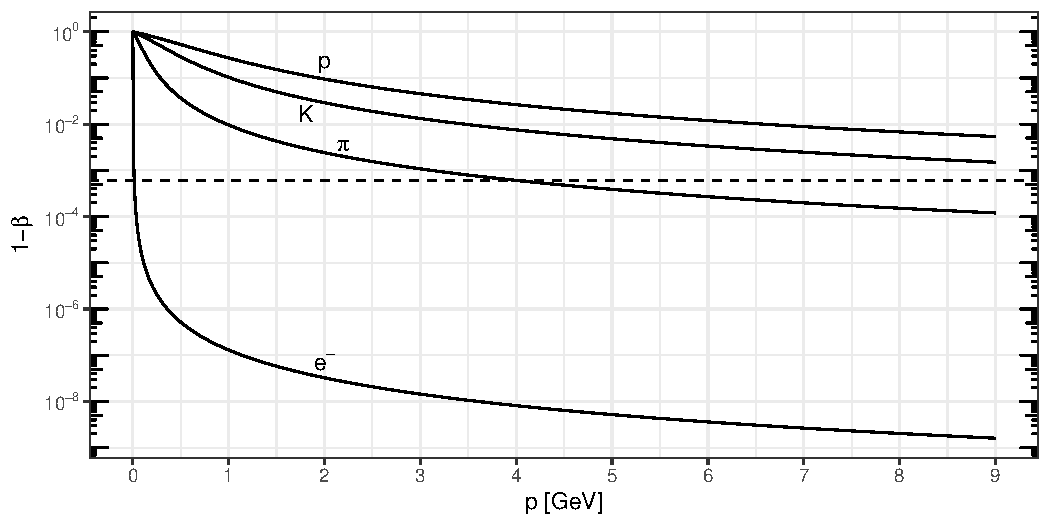
\includegraphics[width=1.0\textwidth]{chap3/hms_cer_threshold.pdf}
    \caption{Value of $1-\beta$ for various particles as a function of
            momentum. The horizontal line represents the Cherenkov threshold
            for \ch{C4F8O} at a pressure of 0.45 atm.
            }
    \label{fig:hms_cer_threshold}
\end{figure}


The gas Cherenkov detectors in the HMS and SHMS use spherical mirrors to focus
Cherenkov radiation onto PMTs that are read out by the DAQ system.

DISCUSS PHOTOELECTRONS

Over a sufficiently narrow range of momenta, only some types of particles will
emit Cherenkov radiation.
Using \ch{C4F8O} at 1 atm, the presence or absence of a signal in the Cherenkov
can be used to determine if the particle that generated a trigger is an
electron or a hadron, provided the momentum range in question is below
$\sim$4 \si{\giga\eV}.
Given knowledge of the expected range of momenta an experiment requires and
what types of backgrounds will need to be removed, one can pick an appropriate
Cherenkov medium based on its index of refraction.

\subsubsection{HMS Cherenkov}
% C4F8O at 0.45 atm.
Allows e/pi separation.

Broken mirror during our runs.

\subsubsection{SHMS Noble Gas Cherenkov}
% CO2 at 1 atm.
Designed for e/pi separation.

\subsubsection{SHMS Heavy Gas Cherenkov}
% CO2 at 1 atm.
Designed for pi/K separation.

\subsubsection{SHMS Aerogel Cherenkov}
Designed for K/p separation.

\subsection{Calorimeters}
A lead glass calorimeter provides another means for discriminating between
electrons and hadrons.
The calorimeters in both spectrometers consist of lead blocks with
PMTs attached that collect light generated by electromagnetic showers.
The electric field of the nuclei in the block will slow down a high energy
electron passing through the block.
The electron will radiate Bremsstrahlung photons, which will in turn generate
positron-electron pairs that will also radiate photons, and so on.
The resulting electromagnetic shower of photons, electrons, and positrons
generates Cherenkov radiation that is collected by PMTs mounted on the ends
of the lead glass blocks.
The amount of light collected is proportional to the deposited energy.
Electrons, positrons, and photons will deposit all of their energy.
For the kinematics of E12-06-102, this is between 2 and 6 GeV.
These particles will produce a peak centered around 1 in the distribution of
the track-normalized energy deposition, $E/p$.
A pion, whose mass is much greater than an electron's, will typically deposit
about 300 MeV.
A negative pion undergoing a charge-exchange reaction in the bulk of the
calorimeter can produce a neutral pion which will decay into two photons,
resulting in a significant fraction of energy being deposited.
As a result, there is a large pion tail in the $E/p$ distribution that extends
up to 1.
Protons, kaons, etc. typically deposit no energy.

\begin{figure}[ht]
    \centering
    \begin{subfigure}[b]{0.35\textwidth}
        \centering
        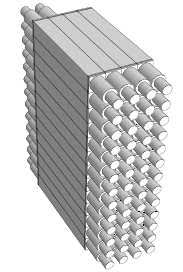
\includegraphics[width=\textwidth]{chap3/hms_calorimeter_drawing_lores.jpg}
        \caption{HMS calorimeter}
        \label{fig:hms_calorimeter}
    \end{subfigure}
    \hfill
    \begin{subfigure}[b]{0.35\textwidth}
        \centering
        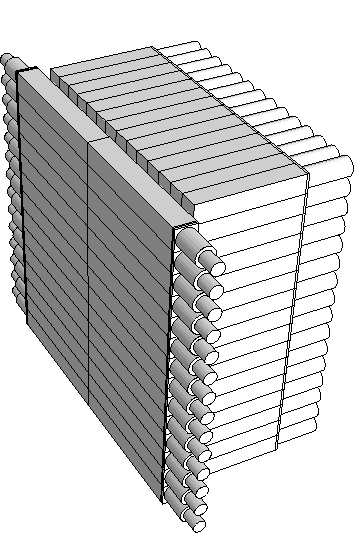
\includegraphics[width=\textwidth]{chap3/shms_calorimeter_drawing.png}
        \caption{SHMS calorimeter}
        \label{fig:shms_calorimeter}
    \end{subfigure}
    \caption{The HMS and SHMS calorimeters}
    \label{fig:calorimeters}
\end{figure}

\subsubsection{HMS Calorimeter}
The HMS calorimeter\cite{Mkrtchyan_2012} consists of four rows of thirteen
10x10x70 \si{\cm\cubed} lead glass blocks.
The total thickness is $\sim$14.6 radiation lengths.
The blocks are made of TF-1 type lead glass with an index of refraction of
1.65, radiation length 2.74 \si{cm}, and density 3.86 \si{\gram\per\cm\cubed}..
Each block is wrapped in 25 \si{\um} thick aluminized Mylar and 40
\si{\um} thick Tedlar type film to block external light.
The light generated in each block is collected by two Phillips XP3462B PMTs,
one on each end.

\subsubsection{SHMS Calorimeter}
The SHMS calorimeter consists of a preshower and shower section.
The preshower radiator consists of one layer of 28 TF-1 type lead glass blocks,
identical to the HMS blocks, stacked in two columns of 14 blocks.
The ``fly eye'' shower array consists of 224 modules from the decommissioned
HERMES detector\cite{Avakian_1998} stacked in 14 columns and 16 rows.
The HERMES blocks are i8.9x8.9x50 \si{\cm\cubed} blocks of F-101 type lead glass with
an index of refraction of 1.65, radiation length 2.78 \si{\cm}, and density
3.86 \si{\gram\per\cm\cubed}.
Each preshower block is read out by one Phillips XP3462B PMT, and each shower
block by one Photonis XP3461 PMT.
